\newpage
\section{Chemische Bindungen} \label{kap:1}
	Festkörpereigenschaften beruhen auf den atomaren Eigenschaften der Bausteinen, ihrer Art der Bindung und die relative Anordnung zueinander.

\subsection{Bindungsenergie, Typen von Bindungen}\label{kap:1_1}
	Bindungen entstehen, wenn sich dadurch die Gesamtenergie der Systems verringert. Die Bindungsenergie ist die Energiedifferenz zwischen Gesamtenergie der Bausteine und dem Kristall:
	\begin{align}
		U_{\text{Bindung}} = \sum_i U_{\text{Baustene,i}}-U_{\text{Kristall}} > 0
	\end{align}
	z.B. $U_{Bindungen}$:  Ar: $ \SI{7}{\kilo\joule\per\mole} $; Na: $ \SI{107}{\kilo\joule\per\mole} $; Si: $ \SI{446}{\kilo\joule\per\mole}$ \\
	Ausbildung einer Bindung von Atomen i und j:
	\begin{center}
		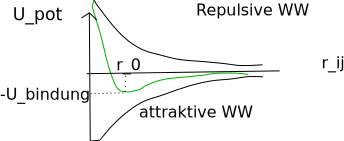
\includegraphics{figures/1_1graph}
	\end{center}
	Beispiel: $U_{pot}^{ij}(r_{ij})= \frac{-a}{r_{ig}^m}+\frac{b}{r_{ij}^n}$ mit $a,b,n,m > 0$ und $n>m$ \newline
	Bindungsenergie:
	\begin{align}
		U_{Bindung} = \frac{1}{2}\sum_i\sum_{i\neq j}U_{pot}(r_0) = \frac{N}{2} \sum_{i\neq j} U_{pot}(r_0)
	\end{align}
	Abschätzung: Coulomb-WW von 2 Ionen $|q| = e$, und $r_0 = 1nm$
	\begin{align}
		U_{pot} \approx \frac{e^2}{4\pi\epsilon\cdot e_0}=\SI{1.4}{\electronvolt} \rightarrow U_{Bindungen} \approx U_{pot} N_A = \SI{140}{\kilo\joule\per\mole}
	\end{align}

\paragraph{Diskussion}
	\begin{itemize}
		\item[1)] attraktive WW: Art der Bindung, vgl. nächste Unterkapitel
		\item[2)] repulsive WW: Atom-Wellenfunktionen dürfen sich nicht vollständig durchdringen aufgrund des Pauli-Prinzips. phänomenologisch: $U_{rep}(r)\approx \frac{1}{r^{12}}$(also n=12)
		\item[3)] NB: Alternative Ansätze: $\approx \frac{1}{r^2}$ mit $6<n<10$
	\end{itemize}

\paragraph{Bindungstypen}
	5 Typen, abhängig von der Elektronenkonfiguration
	\begin{itemize}
		\item[I] \textbf{Van-Der-Waals Bindung:}\newline
			abgeschossene äußere Schale \newline
			Dipol-WW, sehr schwach (0.1eV)\newline
			zum Beispiel Edelgaskristall
		\item[II] \textbf{Ionenbindung:} \newline
			Elektronentransfer $\rightarrow$ Edelgaskonfiguration \newline
			Coulomb-WW, stark (10eV) \newline
			zum Beispiel: NaCl
		\item[III] \textbf{Kovalente Bindung}:\newline
			Überlapp der Elektronenhülle $\rightarrow$  Überlapp der Wellenfunktionen der Valenzelektronen\newline
			$\rightarrow$ gerichtete Bindung \newline
			Coulomb-WW, gerichtet, stark (10eV)\newline
			zum Beispiel Diamant, Silizium
			\begin{center}
				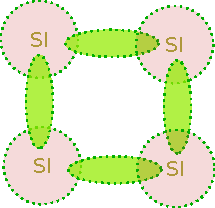
\includegraphics{figures/1_1silizium.pdf}
			\end{center}
		\item[IV] \textbf{metallische Bindung}\newline
			Valenzelektronen komplett delokalisiert, es entsteht \glqq freies Elektronengas\grqq{}
			um die Ionenrümpfe \\
			Coulomb-WW, eher schwach (1eV)\\
			zum Beispiel Na
		\item[V] \textbf{Wasserstoff-Brückenbindung}\newline
			Bindung über ein H-Atom, dass Bindung vermittelt.\newline
			Coulomb-WW, schwach
			\begin{center}
				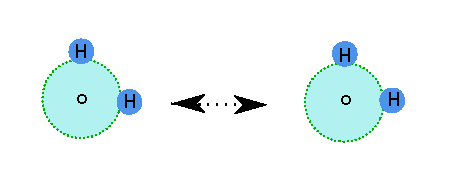
\includegraphics{figures/1_1wasserstoff.pdf}
			\end{center}
			organische Substanzen: DNA Doppelstrang
	\end{itemize}

\subsection{Van-Der-Waals Bindung}\label{kap:1_2}
	Betrachte Atome eines Edelgases mit vollständig besetzten s-und-p-Schalen.
	\begin{itemize}
		\item Kugelsymmetrische Ladungsverteilung
		\item Bindung durch Fluktuationen dieser Ladungsteilungen um den Kern.
		\item Klassische Beschreibung:
			\begin{enumerate}
				\item Verschiebung der Ladungsverteilung in Atomen 1 $\rightarrow$ Dipolmoment $p_1$
				\item Dipol $p_1$ erzeugt elektrisches Feld $E_1$\newline
						Atom 2 im Abstand $r$ von Atom 1:
						\begin{align}
							E_1(r)=\frac{1}{4\pi\epsilon_0}\left(3\frac{p_i r}{r^5}r-\frac{1}{r^3}p_1\right) \
							E_1(r) \propto \frac{p_1}{r^3}
						\end{align}
				\item Atom 2 wird von $E_1$ auch Polarisiert.
						\begin{align}
							P_2 \propto E_1(r) \text{mit Polarisierbarkeit}
							p_2 \propto \frac{p_1}{r^3}
						\end{align}
				\item Elektrisches Feld von Atom 2 am Ort von Atom 1:
						\begin{align*}
							E_2(r) = \frac{1}{4\pi\epsilon_0}\left(3\frac{P_2}{\vec{r}^5}\vec{r}-\frac{1}{\vec{r}^3}p_2\right)
						\end{align*}
				\item Gegenseitige Beeinflussung der Atome stört die kugelsymmetrische Ladungsteilungen, so dass $<p_1>^2 \neq 0$.
				\item Wechselwirkung: $U_{pot}^{12}(r)= -p_2\cdot E_1(r)\propto - \frac{1}{r^6}$
			\end{enumerate}
	\end{itemize}
	Damit: Paarpotential zweier Edelgasatome: \textbf{Lennard-Jones-Potential}
	\begin{align*}
		U_{pot}^{12}=\frac{A}{r^{12}}-\frac{B}{r^6} = e\epsilon\left[\left(\frac{\sigma}{r}\right)^{12} - \left(\frac{\sigma}{r}\right)^{6}\right]
	\end{align*}
	\begin{center}
		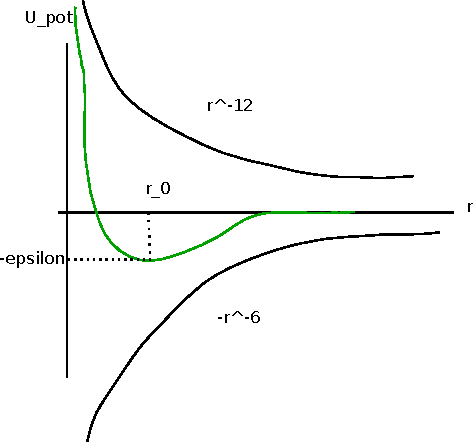
\includegraphics{figures/1_2graph.pdf}
	\end{center}
	mit $\epsilon = \frac{B^2}{4A}$ und $\sigma = \left(\frac{A}{B}\right)^{1/6}$\newline
	und $r_0 = 2^{1/6}\sigma=1.12\sigma$\newline
	Gesamtes WW-Potential des Edelgaskristalls:
	\begin{itemize}
		\item Summation über alle Atome, vgl. Gl 1
		\item Potentialminimum: Gitterabstand $R_0 (\neq r_0)$
	\end{itemize}
	Vergleich: Abschätzung-Experiment:
	\begin{table}[h]
		\centering
		\begin{tabular}{l|llll}
													& Ne & Ar & Kr  & Xe  \\ \hline
			$U_{bidung}^{exp}$ in $\frac{meV}{Atom}$ & 20 & 81 & 116 & 166 \\
			$U_{bidung}$                             & 26 & 89 & 127 & 174 \\
			Korrektur Nullpunktsfluktuation          & -8 & -9 & -7  & -6  \\
			$\sum$                                   & 18 & 80 & 120 & 168
		\end{tabular}
	\end{table}\\
	Was fehlt? Nullpunktsfluktuationen als Unschärferelation $\Delta x\cdot \Delta p \geq \frac{\hbar}{2}$\newline
	Trick: Annäherung von L-J-Pot. nahe $R_0$ durch harmonischen Oszillator \newline
	$\rightarrow \Delta x = \sqrt{\frac{h}{2m\omega}}$

\subsection{Ionische Bindung} \label{kap:1_3}
	Betrachte Atome, die durch Austauch von Elektronen die Edelgaskonfiguration erreichen können.\\
	Bsp.: NaCl
	\begin{itemize}
		\item Na: $1$s$^2 2$s$^2 2$p$^6 3$s$^1 \rightarrow \, \text{Na}^+: \, 1$s$^2 2$s$^2 2$p$^6$
		\item Cl: $1$s$^2 2$s$^2 2$p$^6 3$s$^2 3$p$^5 \rightarrow \, \text{Cl}^-: \, 1$s$^2 2$s$^2 2$p$^6 3$s$^2 3$p$^6$
	\end{itemize}
	\begin{itemize}
		\item[$\rightarrow$] Ionen haben Kugelsymmetrische Ladungsverteilung
		\item[$\rightarrow$] Coulomb-WW (ungerichtet)\\
			Abschätzung: 2 Ionen mit $q = \pm e$ im Abstand $a = 2.8$ \AA:\\ $U_{Coulomb} = -\frac{e^2}{4 \pi \varepsilon_0 a} = - 8.2 \cdot 10^{-19} \text{J} = -5.1 \text{eV}$
	\end{itemize}

	Coulomb-WW ist deutlich stärker als van-der-Waals-WW \\
	(Auch Nullpunktsfunktionen können vernachlässigt werden)\\
	$\rightarrow$ WW im Kristall ist durch WW mit vielen Nachbarionen stärker als die Anschätzung.

\paragraph{Bindungsenergie im Ionenkristall:}
	Verwende 1 aus Kap. \ref{kap:1_1}
	\begin{align*}
		\Phi_i  = \sum_{j \neq i} \left(\pm \frac{Z^2 e^2}{4 \pi \varepsilon_0 r_{ij}} + \frac{A}{r_{ij}^{12}}\right)
	\end{align*}

	Ann: Abstoßende WW ist kurzreichweitig, d.h. nur nächste Nachbarn im Abstand R. Die Zahl der Nächsten Nachbarn $n$ hängt von der Struktur ab.
	\begin{align*}
		\Phi_i                                   & = \sum_{j \neq i} \left(\pm \frac{Z^2 e^2}{4 \pi \varepsilon_0 r_{ij}} + n\frac{A}{R^{12}}\right)
		\qquad \text{mit } r_{ij} = p_{ij} \cdot R                                                                                                                 \\
												& = - \frac{Z^2 e^2}{4 \pi \varepsilon_0 R} \left(\sum_{j \neq i} \frac{\pm 1}{p_{ij}}\right) + n\frac{A}{R^{12}} \\
		\text{Madelung-konstante:} \qquad \alpha & := \left(\sum_{j \neq i} \frac{\pm 1}{p_{ij}}\right)
	\end{align*}
	VZ: +: unterschidliche Ladung; -: gleiches VZ der Ladung.\\
	$\alpha$ hängt von der Kristallstruktur ab. Für NaCl:
	\begin{figure}
		\centering
		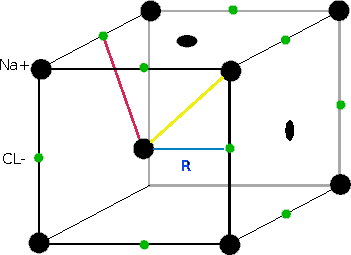
\includegraphics{figures/1_3NaCl.pdf}
		\caption{Vgl. Kap. 2: fcc-Gitter mit 2-atomiger Basis}
	\end{figure}
	jeder Baustein:
	\begin{itemize}
		\item 6 Nachbarn mit $p_{ij} =  1$
		\item 12 Nachbarn mit $p_{ij} =  \sqrt{2}$
		\item 8 Nachbarn mit $p_{ij} =  \sqrt{3}$
	\end{itemize}

	Damit:
	\begin{align}
		\alpha = +6 \cdot \frac{1}{1} - 12 \cdot \frac{1}{\sqrt{2}} + 8 \cdot \frac{1}{\sqrt{3}} - \dots
	\end{align}
	Problem: Reihe ist nur bedingt konvergent. Physikalisch: Oberflächenladung.\\
	Trick: \textbf{Evjen-Methode:} Zerlegung des Kristalls in Zellen mit der Symmetrie des Kristalls, die elektrisch ungeladen sind.
	$\Rightarrow$ Anteilige Zählung von Ladungen an Stirnflächen ($\frac{1}{2}Z$), Kanten ($\frac{1}{4}Z$), Ecken ($\frac{1}{8}Z$).\\
	$\rightarrow$ Für die kleinste Zelle:
	\begin{align}
		\alpha_1 = 6 \cdot \frac{1}{2} \cdot \frac{1}{1}  - 12 \cdot \frac{1}{4} \cdot \frac{1}{\sqrt{2}} + 8 \cdot \frac{1}{8} \cdot \frac{1}{\sqrt{3}} \approx 1.45
	\end{align}
	Madelung-Konstante durch Summation
	\begin{align*}
		\alpha_{NaCl} = \alpha_1 + \alpha_2 + \dots \approx 1.748
	\end{align*}

	Bindungsenergie pro Ionepaar $\Phi_i$
	Gesamte Bindungsenergie: 
	\begin{align} 
		\Phi = \frac{1}{2} \sum_i \Phi_i = \frac{N}{2} \cdot \Phi_i (\text{vgl. Gl. (1)})  \\
		\text{für }\frac{N}{2}\text{ Ionenpaare} \nonumber
	\end{align}
	Gleichgewitszustand $R_0$:
	\begin{align*}
		\frac{\mathrm{d} \varphi}{\mathrm{d} R} = 0 \qquad \text{(Minimierung der pot. Energie)} \\
		\rightarrow \qquad U_{Bindung} = \Phi (R_0) = - \frac{N \alpha Z^2 e^2}{8 \pi \varepsilon_0 R_0} \left(1- \frac{1}{12} \right)
	\end{align*}

	für NaCl: $R_0$ = 2.8 \AA\\
	$U_{Bindung, pro Ionenpaar} = 8.23$ eV\\
	$U_{Bindung,p.I.}^{exp} = 7.95$ eV \\

\paragraph{Chemisch Interpretation der Bindungsenergie:}
	$U_{Bindung} =$ Energie, die Bei Zerlegung des Kristalls in Bausteine aufgewendet werden muß:
	\begin{align*}
		\text{NaCl} \rightarrow \text{Na}^+ + \text{Cl}^-
	\end{align*}
	weiter Energien:
	\begin{itemize}
		\item Ionisierungsenerige des Na $\rightarrow$ Na$^+$ + e$^-$ (5.14 eV)
		\item Elektronenaffinität des Cl + e$^-$ $\rightarrow$ Cl$^-$ (-3.61 eV)
		\item Dissotiation von Cl$_2$ $\rightarrow$ 2Cl
		\item Sublimation von Na-Atomen aus Na-Kristall
	\end{itemize}
(Haber-Born-Kreisprozess)

\subsection{Kovalente Bindung} \label{kap:1_4} %1.4
Betrachte Atome, deren Wellenfunktionen überlappen:
\begin{itemize}
	\item[$\rightarrow$] Entstehung von (Molekül-) Orbitalen, durch die die elektron. Wellenfunktion zwischen den Partnern lokalisiert wird.
	\item[$\rightarrow$] Stark gerichtet, kurzreichweitig, stark
	\item[$\rightarrow$] Moleküle (H$_2$, CH$_4$,\dots), Festkörperphysik (Diamant, Silizium)
	\item[$\rightarrow$] vdW-WW spielt auch in kovalenten Kristallen keine Rolle. 
\end{itemize}
\paragraph{Bestimmung der Bindungsenergie}
$\rightarrow$ IK4, Kap. 17
\paragraph{Bindungsenergie}
Beispiel: \textbf{H$_2^+$-Molekül-Ion}
\begin{figure}[H]
	\centering
	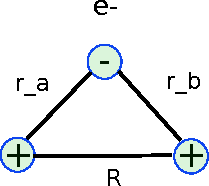
\includegraphics{figures/1_4WasserstoffH2O.pdf}
	\caption{}
	\label{}
\end{figure}
\textbf{Näherungsmethode}: LCAO-Methode (linear combination of atomic orbitals)
\begin{itemize}
	\item Hamilton-Operator: $\hat H = - \frac{\hbar^2}{2m} \Delta - \frac{e^2}{4 \pi \varepsilon_0 r_a} - \frac{e^2}{4 \pi \varepsilon_0 r_b} +\frac{e^2}{4 \pi \varepsilon_0 R}$
	\item SGL: $\hat H \vert\Psi\rangle = E \vert\Psi\rangle$
	\item $\Psi$: Annahme: Für große R hält sich $e^-$ bei Proton a oder b auf und seine Grundzustands-Wellenfunktion ist $\vert\Psi_a\rangle$ oder $\vert\Psi_b\rangle$.\\
\end{itemize}
Für kleinere Abstände R sei $\vert\Psi\rangle = c_1 \vert\Psi_a\rangle + c_2 \vert\Psi_b\rangle$. \\
Damit:
\begin{align*}
	E &= \frac{\langle\Psi\vert\hat{H}\vert\Psi\rangle}{\langle\Psi\vert\Psi\rangle} = \frac{c_1^2 H_{aa} + c_2^2 H_{bb} + 2 c_1 c_2 H_{ab}}{c_1^2 + c_2^2 + 2 c_1 c_2 S}\\
	\text{mit } H_{aa,bb} &= \langle\Psi_{a,b}\vert\hat{H}\Psi_{a,b}\vert\rangle\\  
	H_{ab} &= \langle\Psi_a\vert\hat{H}\vert\Psi_a\rangle = H_{ba}
\end{align*}
Minimierung von $E$ bzgl. $c_1$ und $c_2$:
\begin{align*}
	\frac{\partial E}{\partial c_1} &\stackrel{!}{=} 0 \stackrel{!}{=} \frac{\partial E}{\partial c_2}\\
	\Rightarrow \quad &c_1(H_{aa}-E)+c_2(H_{ab}-E\cdot S) \stackrel{!}{=} 0\\
	&c_1(H_{ab}-E\cdot S)+c_2(H_{bb}-E) \stackrel{!}{=} 0
\end{align*}
\begin{itemize}
	\item[$\rightarrow$] Koeffizientendeterminante verschwindet, falls:
	$$ (H_{aa}-E)(H_{bb}-E) - (H_{ab}-E \cdot S)^2 \stackrel{!}{=} 0 $$
	\item[$\rightarrow$] Mit $H_{aa} = H_{bb}$ : $c_1 = \pm c_2 $
	$$E_{\pm} = \frac{H_{aa} \pm H_{ab}}{1 \pm S} \quad \text{und} \quad \vert\Phi_{\pm}\rangle = c (\vert\Psi_a\rangle \pm \vert\Psi_b\rangle) $$
\end{itemize}
\paragraph{Interpretation}

\begin{figure}[H]
	\centering
	\includegraphics{figures/1_4graph.pdf}
	\caption{}
	\label{}
\end{figure}

\begin{figure}[H]
	\centering
	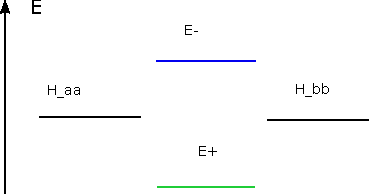
\includegraphics{figures/1_4Energie.pdf}
	\caption{$\rightarrow E_-$ liegt energetisch höher (Antibindendes Orbital \textbf{blau}, bindendes Orbital \textbf{grün})}
	\label{}
\end{figure}
\begin{itemize}
	\item[$\rightarrow$] $\vert\Psi_+\rangle$ ist symmetrisch, d.h. $|\Psi_+|^2$ ist zwischen $a$ und $b$ erhöht.
	\item[$\rightarrow$] $\vert\Psi_-\rangle$ ist antisymmetrisch, d.h. $|\Psi_-|^2$ hat eine Nullstelle zwischen $a$ und $b$.
	\item[$\rightarrow$] $E_+$ ist energetisch günstiger, denn $|\Psi_+|^2$ zwischen $a$, $b$ erhöht $\rightarrow$ Abschwächung der Coulomb-Abstoßung von $a$ und $b$.
\end{itemize}

Systeme mit mehr als 1 Valenzelektron:
\begin{itemize}
	\item zusätzliche Coulomb-Abstoßung der Elektronen
	\item \textbf{Pauli-Prinzip:} Fermionen haben antisymmetrische Gesamt-Wellenfunktion.
	\begin{itemize}
		\item symmetrische Ortswellenfunktion $\vert\Psi\rangle$ und antisymmetrische Spin-Wellenfunktion (Singulett)
		\item antisymmetrische Ortswellenfunktion $\vert\Psi\rangle$ und symmetrische Spin-Wellenfunktion (Triplett)
	\end{itemize}
\end{itemize}
\begin{figure}[]
	\centering
	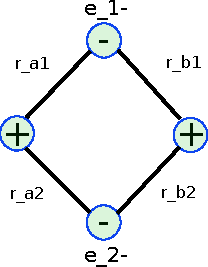
\includegraphics{figures/1_4H2Moleuel.pdf}
	\caption{}
	\label{}
\end{figure}

\textbf{Näherungsmethode}: Heitler-London-Methode\\
Vorgehen analog zu LCAO-Methode, aber mit Zweiteilchen-Welenfunktion.\\
Allgemein Symmetrische/Antisymmetrische Ortswellenfunktion
\begin{align*}
	\Psi_s(\textbf{r}_1,\textbf{r}_2) &\sim (\Psi_a(\textbf{r}_1) + \Psi_b(\textbf{r}_1)) (\Psi_a(\textbf{r}_2) + \Psi_b (\textbf{r}_2))\\
	\Psi_a(\textbf{r}_1,\textbf{r}_2) &\sim (\Psi_a(\textbf{r}_1) - \Psi_b(\textbf{r}_1)) (\Psi_a(\textbf{r}_2) - \Psi_b (\textbf{r}_2))
\end{align*}
Annahme:
\begin{align*}
	\Psi_{s,a}(\textbf{r}_1,\textbf{r}_2) \sim \Psi_a(\textbf{r}_1) \Psi_b (\textbf{r}_2) \pm \Psi_b (\textbf{r}_1) \Psi_a (\textbf{r}_2)
\end{align*}
weiteres Vorgehen analog.
Diskussion:
\begin{itemize}
	\item Lovalente Bindungen nur bei starkem Überlapp der Wellenfunktionen.
	\item Höchstens 2 Elektronen, damit nur bindendes Molekülorbital besetzt wird.
	\item Ortsabhängigkeit der Wellenfunktion $\rightarrow$ Kovalente Bindung nur in bestimten Richtungen im Kristall
\end{itemize}

\textbf{Allgemeiner Ansatz:} Zweiteilchen-Ortswellenfunktion
\begin{align*}
	\Psi_s(\textbf{r}_1,\textbf{r}_2) = \Psi_s(\textbf{r}_1) \Psi_s(\textbf{r}_2) &\sim (\Psi_a(\textbf{r}_1) + \Psi_b(\textbf{r}_1)) (\Psi_a(\textbf{r}_2) + \Psi_b (\textbf{r}_2))\\
	\Psi_a(\textbf{r}_1,\textbf{r}_2) = \Psi_s(\textbf{r}_1) \Psi_A(\textbf{r}_2) &\sim (\Psi_a(\textbf{r}_1) + \Psi_b(\textbf{r}_1)) (\Psi_a(\textbf{r}_2) - \Psi_b (\textbf{r}_2))
\end{align*}

\paragraph{Wichtige Fälle}
\begin{itemize}
	\item[(a)] \textbf{sp$^3$-Hybridisierung: z.B. Diamant}\\
	C: $1$s$^2 \, 2$s$^2 \, 2$p$^2$ $\rightarrow$ 2 kovalente Bindungen?\\
	\begin{itemize}
		\item[$\rightarrow$] Rehybridisierung: größere Bindungsenergie durch 4 kovalente Bindungen. Zerlegung von $2$s$^22$p$^2$ in $2$s$^12$p$_x^12$p$_y^12$p$_z^1$\\
		Bildung von Linearkombinationen (sp$^3$-Orbitale):\\
		$$\Psi_i = \frac{1}{2} (\Psi_S \pm \Psi_{p_x} \pm \Psi_{p_y} \pm \Psi_{p_z}) \quad \text{mit} \quad (+++), (+--), (-+-), (--+)$$
		\item [$\rightarrow$] 4 tetraedisch angeordnete Keulen\\
		\begin{figure}[H]
			\centering
			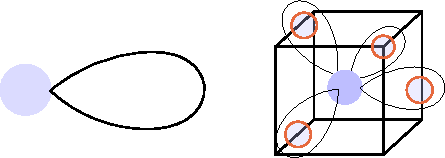
\includegraphics{figures/1_4bindungen.pdf}
			\caption{sp$^3$-Orbital (links) und 4sp$^3$-Orbitale (rechts). Winkel der Kugelwolken $109,5$ deg }
			\label{}
		\end{figure}
		\item[$\rightarrow$] Tetraederstruktur (sp$^3$-Hybridisierung): viele Materialien, z.B. Si, Ge, GaAs,...
	\end{itemize}
	\item[(b)] \textbf{sp$^3$-Hybridisierung}, z.B. Graphen\\
	C:  $1$s$^2 \, 2$s$^2 \, 2$p$^2$\\
	\begin{itemize}
		\begin{figure}[H]
			\centering
			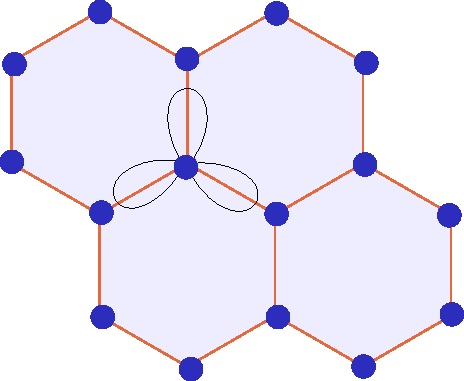
\includegraphics{figures/1_4Kristall.pdf}
			\caption{Winkel 120 deg}
			\label{}
		\end{figure}
		\item[$\rightarrow$] Rehybridisierung: sp$^3$-Orbitale \\
		$2$s$^1$ 2p$_x^1$ 2p$_y^1$ \\ 
		Das übrige 2p$_z$ $\bot$ sp$^2$-Ebene kann $\pi$-Bindungen eingehen (delokalisierte Elektronen), z.B. für Bindungen Graphit $\rightarrow$ Graphit. 
	\end{itemize}
\end{itemize}

\subsection{Metallische Bindung} %1_5
\label{kap:1_5}
\begin{itemize}
	\item[$\rightarrow$] Überlapp von elektronischen Wellenfunktionen, allerdings hier mit vielen Atomen
	\item[$\rightarrow$] Es entsteht ein sogenanntes \textit{freies Elektronengas}, d.h. Valenzelektronen sind delokalisiert.
	\item[$\rightarrow$] Bindung ist ungerichtet und nicht so stark, wie die kovalente Bindung, wg. Abschirmung durch Rümpfe:
	\begin{table}[H]
		\centering
		\begin{tabular}{l|l|l|l|l}
						 & Li   & Na   & Fe   & Co   \\
						 \hline
		$U_{Bidung}$(eV) & 1,63 & 1,11 & 4,28 & 4,39 \\    
		\end{tabular}
		\end{table}
	\textbf{NB:} Übergangsmetalle (d-Elektronen)  haben kovalenten Anteil und daher stärkere Bindungsenergie.
	\item[$\rightarrow$] relativ geringe $U_{Bindung}$ $\rightarrow$ Gitterabstände größer als bei kovalenten o. Ionenkristallen.\\
	$\rightarrow$ Metalle weich, kl.Schmelztemperatur
	\item[$\rightarrow$] hohe elektrische und thermische Leitfähigkeit durch \textit{freie} Valenzelektronen.
\end{itemize}
[Details: erfordern elektronische Eigenschaften von Kristallen]

\subsection{Wasserstoff-Brückenbindung} %1_6
\label{kap:1_6}
Bindung eines H-Atoms an 2 andere Atome, die nicht in \ref{kap:1_2}, \ref{kap:1_3}, \ref{kap:1_4}, \ref{kap:1_5}%TODO: make labels in the according kap's%
passt.\\
$\rightarrow$ H: 1s$^1$ d.h Ionenbindung grundsätzlich möglich, aber $U_{Bindung}$ = 13.6 eV zu stark, genauso für metallische Bindung. Kovalente Bindung möglich. \\
$\rightarrow$ Bindungspartner mit hoher Elektronegativität (z.B. O, N, F): H-Brücke.
\begin{figure}[H]
	\centering
	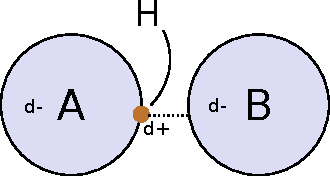
\includegraphics{figures/1_6Wasserstoff.pdf}
	\caption{Valenzelektron des H-Atoms geht fast vollständig auf Bindungspartner A über.\\
	Effektive positive Ladung $\rightarrow$ Bindung an B.\\
	Keine weiteren Bindungspartner aus räumlichen Gründen.}
	$U_{Bindung pro Atom}$ = 0.1 eV (ähnlich wie VDW-Bindung)
	\label{}
\end{figure}

$\rightarrow$ thermische Aktivierung bei Raumtemperatur $\rightarrow$ Biomoleküle\\
typischer Bindungsabstand: 1-2 \AA (also $>>$ vdW-Bindung)\\
z.B. H$_2$O ($\rightsquigarrow$ Dichteanomalie), DNA Doppelhelix
